%************************************************
\chapter{Introduction}\label{ch:introduction}
%************************************************

\begin{quote}
Problem-solvers must find relevant data.  How does the human mind
retrieve what it needs from among so many millions of knowledge items?
Different AI systems have attempted to use a variety of different
methods for this.  Some assign keywords, attributes, or descriptors to
each item and then locate data by feature-matching or by using more
sophisticated associative data-base methods.  Others use
graph-matching or analogical case-based adaptation.  Yet others try to
find relevant information by threading their ways through systematic,
usually hierarchical classifications of knowledge---sometimes called
``ontologies''.  But, to me, all such ideas seem deficient because it
is not enough to classify items of information simply in terms of the
features or structures of those items themselves.  This is because we
rarely use a representation in an intentional vacuum, but we always
have goals---and two objects may seem similar for one purpose but
different for another purpose.
\end{quote}
\begin{flushright}
 --- \defcitealias{minsky:1991}{Marvin Minsky}\citetalias{minsky:1991} \citep{minsky:1991}
\end{flushright}

\section{Two Popular Approaches to Modelling Intelligence}

Recently, there have been two directions of research with the goal of
building a machine that explains intelligent human behavior.  The
first approach is to build a baby-machine that learns from scratch to
accomplish goals through interactions with its environment.  The
second approach is to give the machine an abundance of knowledge that
represents correct behavior.

Each of these solutions has benefits and drawbacks.  The baby-machine
approach is good for dealing with novel problems, but these problems
are necessarily simple because complex problems require a lot of
background knowledge.  The data abundance approach deals well with
complicated problems requiring a lot of background knowledge, but
fails to adapt to changing environments, for which the algorithm has
not already been trained.

\section{The Commonsense Reasoning Problem Domain}

Commonsense reasoning is a long-standing goal of the field of
artificial intelligence.  One of the difficulties in developing
algorithms for dealing with a commonsense reasoning domain is that the
algorithm needs a lot of background knowledge about a given domain
before it can answer even simple questions about it.  However, this
knowledge is often only true in very specific situations and has many
exceptional cases.  For example, the knowledge that most birds can fly
is generally true, but we also know that many birds are flightless,
such as penguins, ostriches, and road runners.  Also, we have
knowledge about the typical behavior of objects; for example, we know
that refridgerators keep things cold, but we also reason efficiently
about exceptional cases, such as when the refridgerator is not plugged
in, or when the power goes out.

\subsection{The Valley of Complex Adaptability}

We would like to build intelligent machines that are able to perform
household tasks, such as cooking, cleaning, and doing the laundry, but
these tasks seem deep within the ``valley of complex adaptability''.


\subsection{Representations for Commonsense Reasoning}

There have been many approaches to artificial intelligence that use
first-order logic as a representation for these types of knowledge and
their exceptions, but these systems become cumbersome in their
inability to express ``fuzzy'' sorts of relationships, such as when
the knowledge is applicable, for example the modifiers, ``most of the
time'', ``usually'', and ``almost never'', are difficult to express in
first-order logic.  When we have a lot of knowledge, we need ways to
keep track of in which situations this knowledge is useful.  This is a
form of ``meta-knowledge'', or knowledge about knowledge.
Meta-knowledge about first-order logic cannot be expressed in
first-order logic, so logic fails us in this regard.  Therefore, we
need other ways to represent our knowledge in addition to logic.

\subsection{The Origins of Knowledge}

If we are going to be clear about what we mean by meta-knowledge, we
first must be more precise about what we mean by knowledge in the
first place.

\subsection{The Reinforcement Learning Model}

Figure~\ref{fig:agent_environment} shows the basic reinforcement
learning model.  In this model, we make a distinction between a
computational process that is the environment and a computational
process that is the agent.  These two processes communicate
information along three channels: (1) an action channel from the agent
to the environment, (2) a perception channel from the environment to
the agent, and (3) a reward channel from the environment to the agent.

\begin{figure}[bth]
  \center
  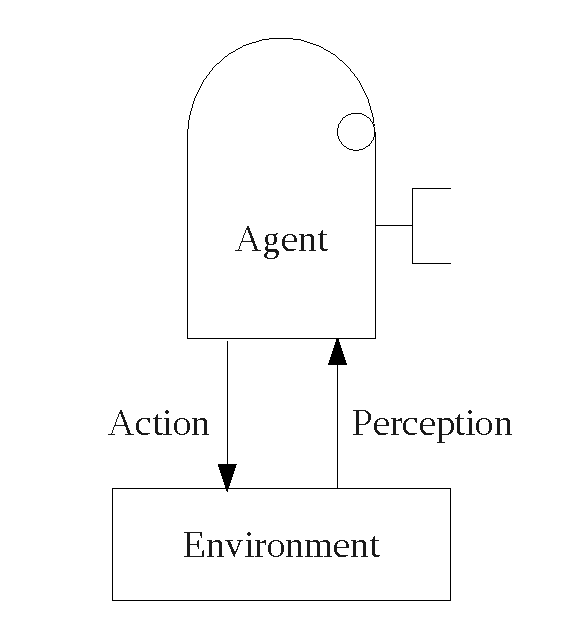
\includegraphics[width=4cm]{gfx/agent_environment}
  \caption[The reinforcement learning model]{The reinforcement learning model.}
  \label{fig:agent_environment}
\end{figure}

The reinforcement learning model is a useful model because it is one
of the simplest formulations of goal-oriented learning.
Figure~\ref{fig:perception_categorization} shows how the simplest
types of categorizations of perceptions can be learned.  Note that any
categorization is more or less useful to us based on how well it
approximates the reward function.

\begin{figure}[bth]
  \center
  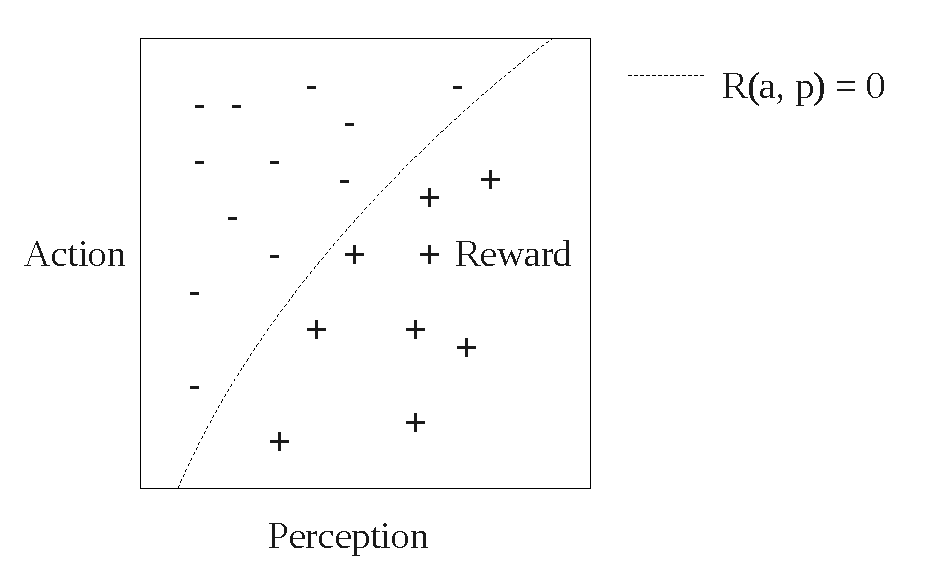
\includegraphics[height=4cm]{gfx/perception_categorization}
  \caption[Categorizing perceptions and actions by knowing rewards]{Categorizing perceptions and actions by knowing rewards.}
  \label{fig:perception_categorization}
\end{figure}




\subsection{Layers of Knowledge about Knowledge}



\section{Using Background Knowledge in a Goal-Oriented Domain}

We are working on an algorithm that benefits from both of these
approaches by learning from cultural language knowledge, while
reflectively monitoring and recognizing the failures of this knowledge
when it is used in a goal-oriented domain.

\section{A New Lisp Programming Language for Modern Computer Architectures}

Toward this end we have developed a reflective programming language
allowing us the ability to monitor the execution and interactions
between large numbers of complicated lisp-like processes.

\section{A Reflective Cognitive Architecture for Layering Failure Tolerant Control Algorithms}

Further, we have developed a cognitive architecture within our
language that provides structures for layering reflective processes,
resulting in a hierarchy of control algorithms that respond to
failures in the layers below.

\section{A Demonstration in a Social Commonsense Reasoning Domain}

Finally, we present an example of our cognitive architecture learning
in the context of a social commonsense reasoning domain with parents
that teach children as they attempt to accomplish cooking tasks in a
kitchen.

